\documentclass[10pt,a4paper]{amsart}
\usepackage[margin=19mm]{geometry}
\usepackage{amsmath,amssymb,mathtools}
\usepackage[scr=rsfs,cal=euler]{mathalfa}
\usepackage{xfrac}
\usepackage[unicode,hidelinks,bookmarks=false]{hyperref}
\newcommand{\ie}{i.e.\ }
\newcommand{\cf}{cf.\ }
\newcommand{\resp}{respectively\ }
\newcommand{\Subsection}{\subsection}
\providecommand{\nobreakdash}{\nobreak\hbox{-}}
\setlength{\emergencystretch}{2em}
\multlinegap0pt
\usepackage{tikz}
\usepackage{xcolor}
\usepackage{amssymb}
\usepackage{enumerate}
\usepackage{float}
\usepackage[normalem]{ulem}
\newtheorem{lemma}{Lemma}
\newtheorem{claim}{Claim}
\title{Minimum degree conditions for removable matchings in $k$-connected graphs}
\author{Hojin Chu, Ringi Kim,, Boram Park}
\date{Source: arXiv:2607.17533v1 (CC BY 4.0)}
\begin{document}
\maketitle

\noindent\emph{Source and licence.} Minimum degree conditions for removable matchings in $k$-connected graphs. Version arXiv:2607.17533v1 (CC BY 4.0), distributed by arXiv under the Creative Commons Attribution 4.0 International licence, http://creativecommons.org/licenses/by/4.0/, as recorded in the arXiv licence metadata for this exact version and shown on the abstract page https://arxiv.org/abs/2607.17533v1. Full licence notice: \texttt{licenses/arxiv-2607.17533-CC-BY-4.0.txt}.\par\smallskip

\noindent\textit{Editorial scope.} Counted unit: the article's claim clm:no\_neighbor\_ATU (source0.tex lines 465--467). The article's complete original proof of it is delivered with it (source0.tex lines 468--567, one \texttt{proof} environment of 100 lines). No mathematics is written, repaired or re-derived: the statement and the proof are the article's own lines, in the article's own notation, and no retained line is substituted or re-flowed.  Retained uncounted as the source-local context the proof needs: lines 291--305; lines 309--360.  Nothing was omitted from any retained span, so the package carries no omission record.  No retained line contains a citation, so the wrapper carries no bibliography and no bibliography entry.  The retained lines contain the article's own diagram code, which the wrapper typesets with the standard tikz packages; no image file is delivered and the package declares no asset dependency.  Editorial formatting only, in addition: an AMS \texttt{amsart} preamble that restates the article's own declarations and macros used by the retained lines, namely the environments \texttt{lemma}, \texttt{claim} on separate counters, together with the standard packages those lines need.  The retained environments print in this document as Lemma 1, Claim 1 in order of appearance, whereas the article prints the same items with the numbering of its own full document.  The complete native source of the article as distributed in the arXiv e-print for this exact version is bundled unchanged as \texttt{sources/205578/source0.tex}.
\begin{lemma}\label{lem:uncrossing}
Let $H$ be a $k$-connected graph for a positive integer $k$.
Suppose that $(u,v,T,A,B)$ and $(u',u,T',A',B')$ are witnesses for two distinct non-$k$-removable edges $uv,\,u'u\in E(H)$. 
Define
\[
  T_1=T\cap A',\quad T_2=T\cap B',\quad T'_1=T'\cap A,\quad T'_2=T'\cap B,
\]
and, for $i,j\in\{1,2\}$, set $Q_{ij}=(T\cap T')\cup T_i\cup T'_j$ (see
Figure~\ref{fig:crossing-witnesses}). 
Then the following hold.
\begin{itemize}
\item[(i)] If $|Q_{21}|\le k-2$, then $d_H(u)\le k$.
\item[(ii)] If $|Q_{21}|\ge k-1$, then $B\cap A'=\emptyset$. In addition, if $|Q_{11}|\ge k$, then $B\cap B'=\emptyset$, $|A|>|B|$, and $|A|>|A'|$ or $|A|>|B'|$.
\end{itemize}
\end{lemma}

\begin{figure}[ht]
\centering
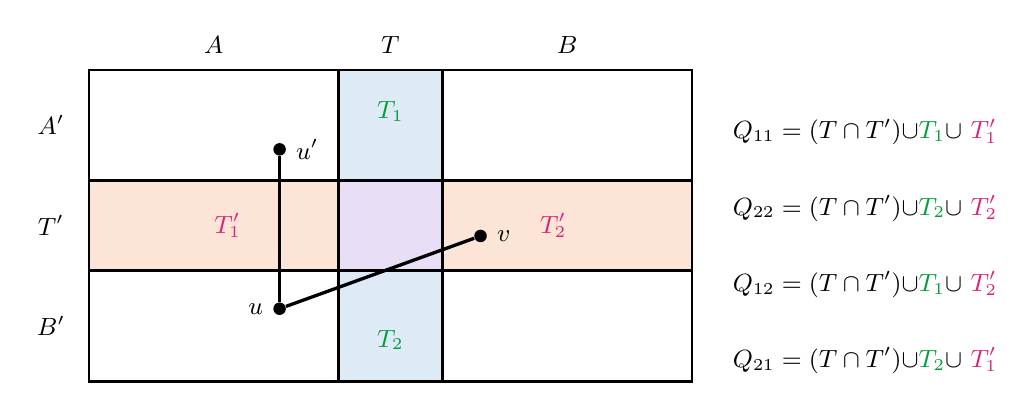
\begin{tikzpicture}[scale=0.88, every node/.style={font=\small}]
\definecolor{cutblue}{RGB}{222,235,247}
\definecolor{cutred}{RGB}{252,228,214}
\definecolor{overlappurple}{RGB}{232,222,245}
\definecolor{qmagenta}{RGB}{214,39,120}
\definecolor{qgreen}{RGB}{0,158,60}
% shaded cuts
\fill[cutblue] (3.6,1.0) rectangle (5.1,5.5);
\fill[cutred]  (0,2.6) rectangle (8.7,3.9);
\fill[overlappurple] (3.6,2.6) rectangle (5.1,3.9);
% grid
\draw[thick] (0,1.0) rectangle (8.7,5.5);
\draw[thick] (3.6,1.0) -- (3.6,5.5);
\draw[thick] (5.1,1.0) -- (5.1,5.5);
\draw[thick] (0,2.6) -- (8.7,2.6);
\draw[thick] (0,3.9) -- (8.7,3.9);
% column / row labels
\node at (1.8,5.85) {$A$};
\node at (4.35,5.85) {$T$};
\node at (6.9,5.85) {$B$};
\node at (-0.55,4.7)  {$A'$};
\node at (-0.55,3.25) {$T'$};
\node at (-0.55,1.8)  {$B'$};
% vertices and edges
\node[circle,fill=black,inner sep=1.6pt,label=right:$u'$] (up) at (2.75,4.35) {};
\node[circle,fill=black,inner sep=1.6pt,label=left:$u$]  (u)  at (2.75,2.05) {};
\node[circle,fill=black,inner sep=1.6pt,label=right:$v$] (v)  at (5.65,3.1) {};
\draw[very thick] (u) -- (v);
\draw[very thick] (up) -- (u);
% region labels
\node[qmagenta] at (2.0,3.25) {$T'_1$};
\node[qmagenta] at (6.7,3.25) {$T'_2$};
\node[qgreen]   at (4.35,4.9) {$T_1$};
\node[qgreen]   at (4.35,1.6) {$T_2$};
% Q legend
\node[align=left,anchor=west] at (9.15,4.6)
    {$Q_{11}=(T\cap T')\cup$\textcolor{qgreen}{$T_1$}$\cup$ \textcolor{qmagenta}{$T'_1$}};
\node[align=left,anchor=west] at (9.15,3.5)
  {$Q_{22}=(T\cap T')\cup$\textcolor{qgreen}{$T_2$}$\cup$ \textcolor{qmagenta}{$T'_2$}};
\node[align=left,anchor=west] at (9.15,2.4)
 {$Q_{12}=(T\cap T')\cup$\textcolor{qgreen}{$T_1$}$\cup$ \textcolor{qmagenta}{$T'_2$}};
\node[align=left,anchor=west] at (9.15,1.3)
  {$Q_{21}=(T\cap T')\cup$\textcolor{qgreen}{$T_2$}$\cup$ \textcolor{qmagenta}{$T'_1$}};
\end{tikzpicture}
\caption{The two witnesses $(u,v,T,A,B)$ and $(u',u,T',A',B')$. The vertical
strip is the vertex cut $T$ in $H-uv$, and the horizontal strip is the vertex cut
$T'$ in $H-u'u$. The vertex $u'$ lies in $A'$ and outside $B$; it may lie in $A$
or in $T$.}
\label{fig:crossing-witnesses}
\end{figure}

\begin{claim}\label{clm:no_neighbor_ATU}
$u$ has no neighbor in $(A\cup T)\cap U$.
\end{claim}

\begin{proof} Suppose that $u$ has a neighbor in $(A\cup T) \cap U$.
If $u$ has a neighbor in $A\cap U$, then choose a neighbor $u'$ of $u$ in $A\cap U$.
Otherwise, let $u'$ be a neighbor of $u$ in $T\cap U$.
As $u'u\in E(H[U])$ is not $k$-removable, there is a witness $(u',u,T',A',B')$ for $u'u$. 
We adopt the notation in Lemma~\ref{lem:uncrossing}.
We first show that $B\cap A'=A\cap A'=\emptyset$, and so $u'\in T_1$, as shown in  Figure~\ref{fig:crossing-witnesses2}.  

 

\begin{figure}[ht]
\centering
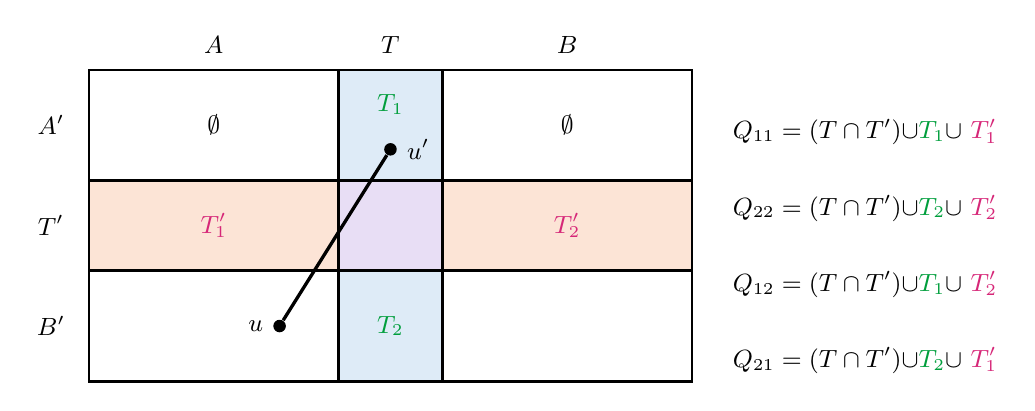
\begin{tikzpicture}[scale=0.88, every node/.style={font=\small}]
\definecolor{cutblue}{RGB}{222,235,247}
\definecolor{cutred}{RGB}{252,228,214}
\definecolor{overlappurple}{RGB}{232,222,245}
\definecolor{qmagenta}{RGB}{214,39,120}
\definecolor{qgreen}{RGB}{0,158,60}
% shaded cuts
\fill[cutblue] (3.6,1.0) rectangle (5.1,5.5);
\fill[cutred]  (0,2.6) rectangle (8.7,3.9);
\fill[overlappurple] (3.6,2.6) rectangle (5.1,3.9);
% grid
\draw[thick] (0,1.0) rectangle (8.7,5.5);
\draw[thick] (3.6,1.0) -- (3.6,5.5);
\draw[thick] (5.1,1.0) -- (5.1,5.5);
\draw[thick] (0,2.6) -- (8.7,2.6);
\draw[thick] (0,3.9) -- (8.7,3.9);
% column / row labels
\node at (1.8,5.85) {$A$};
\node at (4.35,5.85) {$T$};
\node at (6.9,5.85) {$B$};
\node at (-0.55,4.7)  {$A'$};
\node at (-0.55,3.25) {$T'$};
\node at (-0.55,1.8)  {$B'$};
% empty corner cells
\node at (1.8,4.7) {$\emptyset$};
\node at (6.9,4.7) {$\emptyset$};
% vertices and edge
\node[circle,fill=black,inner sep=1.6pt,label=right:$u'$] (up) at (4.35,4.35) {};
\node[circle,fill=black,inner sep=1.6pt,label=left:$u$]  (u)  at (2.75,1.8) {};
\draw[very thick] (up) -- (u);
% region labels
\node[qmagenta] at (1.8,3.25) {$T'_1$};
\node[qmagenta] at (6.9,3.25) {$T'_2$};
\node[qgreen]   at (4.35,5) {$T_1$};
\node[qgreen]   at (4.35,1.8)   {$T_2$};
% Q legend
\node[align=left,anchor=west] at (9.15,4.6)
    {$Q_{11}=(T\cap T')\cup$\textcolor{qgreen}{$T_1$}$\cup$ \textcolor{qmagenta}{$T'_1$}};
\node[align=left,anchor=west] at (9.15,3.5)
  {$Q_{22}=(T\cap T')\cup$\textcolor{qgreen}{$T_2$}$\cup$ \textcolor{qmagenta}{$T'_2$}};
\node[align=left,anchor=west] at (9.15,2.4)
 {$Q_{12}=(T\cap T')\cup$\textcolor{qgreen}{$T_1$}$\cup$ \textcolor{qmagenta}{$T'_2$}};
\node[align=left,anchor=west] at (9.15,1.3)
  {$Q_{21}=(T\cap T')\cup$\textcolor{qgreen}{$T_2$}$\cup$ \textcolor{qmagenta}{$T'_1$}};
\end{tikzpicture}
\caption{The two witnesses $(u,v,T,A,B)$ and $(u',u,T',A',B')$ in the proof of Claim~\ref{clm:no_neighbor_ATU}.}
\label{fig:crossing-witnesses2}
\end{figure}

If $|Q_{21}|\le k-2$, then $A\cap B'=\{u\}$ since  otherwise $Q_{21}\cup\{u\}$ would be a vertex cut of size at most $k-1$ 
separating $v$ from $(A\cap B') -\{u\}$. However, this also yields a contradiction since $d_H(u)\le |Q_{21}\cup\{u',v\}|\le k$.
Thus $|Q_{21}|\ge k-1$.
By Lemma~\ref{lem:uncrossing}(ii), $B\cap A'=\emptyset$.

Suppose to the contrary that $A\cap A'\neq \emptyset$. Suppose $|Q_{11}|\ge k$.
By Lemma~\ref{lem:uncrossing}(ii) again, $B\cap B'=\emptyset$ and $|A|>|B|$.
Then the witness $(v,u,T,B,A)$ satisfies $|B|<|A|$, so by the minimality of $|A|$ it is not a good witness, that is, $|W\cap B|\ge\lfloor w/2\rfloor+1$. Hence
\[
   |W\cap(A\cup T)|=|W|-|W\cap B|
   \le w-\Bigl(\Bigl\lfloor\tfrac w2\Bigr\rfloor+1\Bigr)
   \le \Bigl\lfloor\tfrac w2\Bigr\rfloor .
\]
Since $B\cap A'=B\cap B'=\emptyset$, we have $|W\cap A'|\le\lfloor w/2\rfloor$ and $|W\cap B'|\le\lfloor w/2\rfloor$. 
Thus both $(u',u,T',A',B')$ and $(u,u',T',B',A')$ are good.
Then the minimality of $|A|$ yields $|A|\le|A'|$ and $|A|\le|B'|$, contradicting Lemma~\ref{lem:uncrossing}(ii).
Hence $|Q_{11}|\le k-1$.
If $u'\in A$, $Q_{11}$ gives a good witness for $u'u$, which contradicts the minimality of $|A|$. 
If $u' \not\in A$, then $Q_{11}$ is a vertex cut of $H$, which contradicts the $k$-connectedness of $H$.
Therefore $A\cap A'=\emptyset$, which implies that $u' \in T$.

Since $A'=T_1$ and $d_H(u')\ge h(k,w)\ge k+\lceil (w+1)/4\rceil$, 
it follows that $N_H(u')\subseteq (T_1\setminus\{u'\})\cup T'\cup\{u\}$, and we obtain 
\[
   |T_1|\ge |N_H(u')\cap T_1|+1\ \ge\ d_H(u')-|T'|\ \ge\ \Bigl\lceil \tfrac{w+1}{4}\Bigr\rceil+1.
\]
Since $u' \in T$, it follows that $u$ has no neighbor in $A\cap U$ by the choice of $u'$.
Note that $uu'$ is the only edge joining $A'$ and $B'$ in $H-T'$.
Thus no vertex in $T_1-\{u'\}$ is adjacent to $u$, so 
\[
   N_H(u)\ \subseteq\ (A\cap W) \cup \bigl(T\setminus T_1 \bigr) \cup \{u', v\} .
\]
Hence, since $(u,v,T,A,B)$ is good and $|T|=k-1$,
\[
   d_H(u)\ \le\ \Bigl\lfloor\tfrac w2\Bigr\rfloor
              +\Bigl((k-1)-\Bigl\lceil \tfrac{w+1}{4}\Bigr\rceil-1 \Bigr)+2
          \ =\ k+\Bigl\lfloor\tfrac w2\Bigr\rfloor-\Bigl\lceil \tfrac{w+1}{4}\Bigr\rceil < k+\Bigl\lceil \tfrac{w+1}{4}\Bigr\rceil \le h(k,w),
\]
a contradiction. 
\end{proof}

\end{document}
